\subsection{CSS 3}

\citeonline{silva_css_3} afirma que a principal função do \textit{Cascading Style Sheet} - CSS\footnotemark[28] - é definir como os componentes anteriormente estruturados nos documentos \textit{web}, por meio do HTML, devem ser apresentados ao usuário.

\footnotetext[28]{CSS: \textit{Cascading Style Sheet} - Documentos que definem estilos aos componentes da página \textit{web}.}

Para \citeonline{w3c_css_definition}, o CSS é "\textit{a simple mechanism for adding style (e.g., fonts, colors, spacing) to Web documents}\footnotemark[29]".

\footnotetext[29]{O CSS é um simples mecanismo para adicionar estilo, como: fontes, cores, espaços para os documentos \textit{Web}.}

Tim Berners-Lee inicialmente escrevia as estilizações de seus documentos \textit{web}, mesmo que de forma simples e limitada, nos próprios documentos HTML. Isto se deve ao fato de, ele acreditar que tal função deveria ser realizada pelos navegadores. Entretanto, em 1994 a primeira proposta de criação do CSS surgiu e, em 1996, a primeira versão do CSS denominada CSS 1 foi lançada como recomendação do W3C \cite{silva_css_3}.

De acordo com \citeonline{silva_css_3}, atualmente o CSS possui quatro versões, são elas: A CSS 1, a 2, a 2.1 e atualmente a 3, que foi utilizada para o desenvolvimento deste trabalho.

Há três formas de incorporar o CSS em seu documento web segundo \cite{silva_css_3}, são elas: 

\begin{itemize}
	\item \textbf{\textit{Inline}:} É possível aplicar o estilo diretamente ao componente desejado, por meio do uso da propriedade \texttt{style} do componente HTML. Como é apresentado no Código~\ref{list:css_inline};
	
	% Inserindo o código HTML via listagem
	\begin{lstlisting} [style=custom_HTML,caption={[Exemplo de inclusão do estilo CSS \textit{inline}]{Exemplo de inclusão do estilo CSS \textit{inline}. \textbf{Fonte:} Elaborado pelos autores.}}, label=list:css_inline] 	
	<!DOCTYPE html>
		<html>
		<head>
			<title>Titulo da pagina</title>
		</head>
		<body>
			<p style="color:red;">
				Exemplo de estilo CSS aplicado diretamente ao componente
			</p>
		</body>
	</html>
	\end{lstlisting}
	
	% Removido pois não utilizará mais figura e sim listagem
	%\begin{figure}[h!]
	%	\centerline{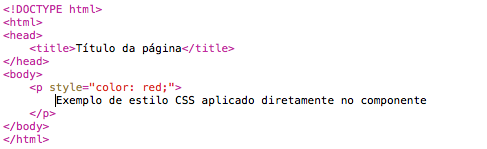
\includegraphics[scale=0.8]{./imagens/example_css_inline.png}}
	%	\caption[Exemplo de inclusão do estilo CSS inline]
	%	{Exemplo de inclusão do estilo CSS inline. \textbf{Fonte:} Elaborado pelos autores.}
	%	\label{fig:css_inline}
	%\end{figure}
	
	\item \textbf{Incorporado:} Outra forma, é escrever todo CSS referente ao  documento \textit{web} dentro da \textit{tag} \texttt{style} do documento HTML. Para tanto, esta \textit{tag} deve ser inserida entre o início e o fim da \textit{tag} \texttt{head} do documento. Como é apresentado no Código~\ref{list:css_incorporado};
	
	% Inserindo o código HTML via listagem
	\begin{lstlisting} [style=custom_HTML,caption={[Exemplo de inclusão do estilo CSS incorporado à página HTML]{Exemplo de inclusão do estilo CSS incorporado à página HTML. \textbf{Fonte:} Elaborado pelos autores.}}, label=list:css_incorporado] 	
	<!DOCTYPE html>
	<html>
		<head>
			<title>Titulo da pagina</title>
			<style>
				p {
					color: red;
				}
			</style>
		</head>
		<body>
			<p>
				Exemplo de estilo CSS aplicado a pagina HTML por meio da TAG style
			</p>
		</body>
	</html>
	\end{lstlisting}
	
	% Removido pois não utilizará mais figura e sim listagem
	%\begin{figure}[h!]
	%	\centerline{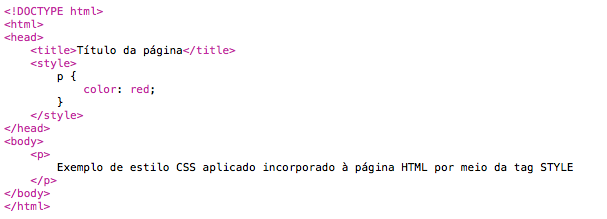
\includegraphics[scale=0.65]{./imagens/example_css_incorpored.png}}
	%	\caption[Exemplo de inclusão do estilo CSS incorporado à página HTML]
	%	{Exemplo de inclusão do estilo CSS incorporado à página HTML. \textbf{Fonte:} Elaborado pelos autores.}
	%	\label{fig:css_incorporado}
	%\end{figure}
	
	\item \textbf{Externo:} A última forma, é criar um arquivo externo com extensão \texttt{.css} e definir todas as regras de estilização do documento \textit{web} neste arquivo. Desta forma, para vincular tal arquivo a um documento HTML específico será necessário utilizar a \textit{tag} \texttt{link} entre o início e o fim da \textit{tag} \texttt{head} do documento, como apresentado no Código~\ref{list:css_externo};
	
	% Inserindo o código HTML via listagem
	\begin{lstlisting} [style=custom_HTML,caption={[Exemplo de inclusão do estilo CSS a partir de um arquivo externo]{Exemplo de inclusão do estilo CSS a partir de um arquivo externo. \textbf{Fonte:} Elaborado pelos autores.}}, label=list:css_externo] 	
	<!DOCTYPE html>
	<html>
		<head>
			<title>Titulo da pagina</title>
			<link rel="stylesheet" href="style.css">
		</head>
		<body>
			<p>
				Exemplo de estilo CSS carregado a partir de um arquivo externo
			</p>
		</body>
	</html>
	\end{lstlisting}
	
	% Removido pois não utilizará mais figura e sim listagem
	%\begin{figure}[h!]
	%	\centerline{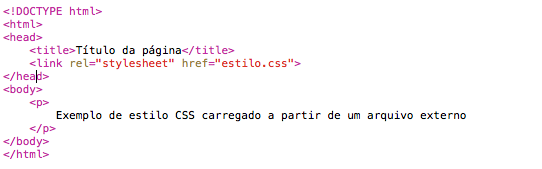
\includegraphics[scale=0.8]{./imagens/example_external_css.png}}
	%	\caption[Exemplo de inclusão do estilo CSS a partir de um arquivo externo]
	%	{Exemplo de inclusão do estilo CSS a partir de um arquivo externo. \textbf{Fonte:} Elaborado pelos autores.}
	%	\label{fig:css_externo}
	%\end{figure}
	
\end{itemize}

O CSS 3 será utilizado neste trabalho, pois, ele permite definir estilos aos componentes das páginas \textit{web} e possui recursos que não são existem em suas versões anteriores, o que nos permite desenvolver páginas mais atrativas com menos recursos.